\section{Hardware}
Das Endprodukt setzt sich hauptsächlich aus dem Melde- und Sensor-Print zusammen. Die Anforderungen der Prints ist es, eine Datenübertragung von den einzelnen Panels      über eine Powerline zu einer Zentrale zu gewährleisten. Zudem muss der Sensorprint kompackt sein und an jedem Pannel montierbar sein.

In den nachfolgenden Kapiteln werden alle Teilschaltungen beschrieben um einen möglichen Nachbau zu erleichtern.

\subsection{Sensorprint}


Jedes Solarpanel wird mit einem Sensorprint auf der Rückseite des Pannels bestückt. Der Sensorprint hat eine grösse von 6 x 6cm und passt somit optimal in die vorgesehene Halterung auf der Rückseite des Pannels eingebaut werden. Als Vorlage für die grösse der Halterung, wurde das Austellemodell im Labor in betracht gezogen.

Der Aufbau des Sensorprints besteht aus einem Mikrocontroller, einem Powerline - Transceiver, einem ADC - Converter und einer 12V - Speisung. Seine Aufgabe ist die Spannungswerte des Solarpannels einzulesen, diese zu verarbeiten und die Informationen über die Powerline an den Meldeprint zu übermitteln. Eine grobe Übersicht über den Aufbau und das Zusammenspielen der einzelnen Komponenten gibt die nachfolgende Abbildung.

\begin{figure}[h]
\centering
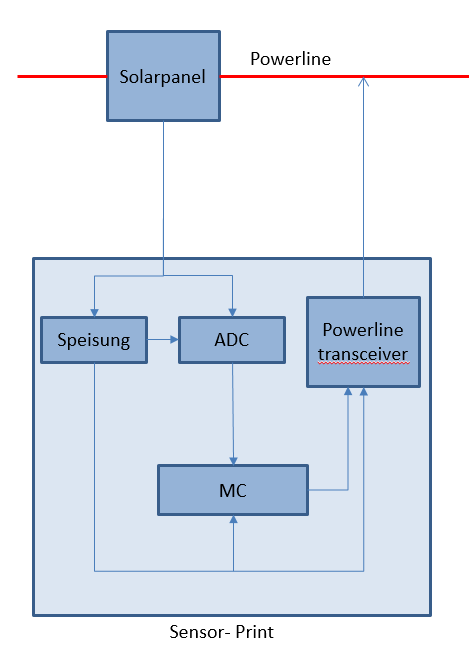
\includegraphics[width=0.5\textwidth]{konzept_sensor}
\caption{Grobkonzept des Sensorprints}
\end{figure}

\subsubsection{Speisung}
Die Speisung des Sensorprints erfolgt über einen LM 2594 DC/DC Regulator. Dieser erhält eine variable Eingangsspannung von 12V - 60V vom Solarpannel. Der DC/DC Regulator regelt diese Eingangsspannung mit hilfe eines Schaltreglers auf eine feste 12V DC Spannung am Ausgang. Diese Spannung gewährleistet die Versorgung des Powerline Transceivers. Die restlichen Elemente werden mit 5V gespiesen.

Die 5V DC Spannung wurde anders als geplannt realisiert. Auf dem Print war nur Platz für eine Speiseschaltung vorgesehen, darum musste die 5V Spannung über den 5V Ausgang des Powerline Transceivers realisiert werden. Da nur eine sehr geringe Leistungen auf dem Sensorprint vorhanden ist, ist diese Beschaltung vertretbar.

In der nachfolgenden Abbildung ist die Beschaltung der 12V Speisung ersichtlich.


\begin{figure}[h]
\centering
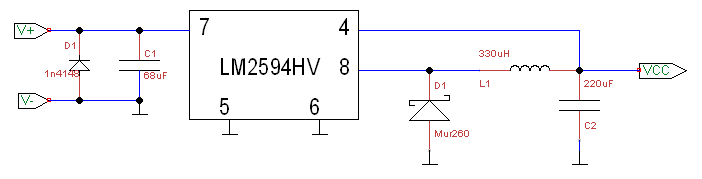
\includegraphics[width=1\textwidth]{speisung_sensor}
\caption{Beschaltung der 12V - Speisung}
\end{figure}

Die ersichtlichen Bauteile wurden anhand der Datenbalttvorgaben des LM2594 ausgewählt.

\
\
\subsubsection{Spannungsmessung}
Die Spannungsmessung erfolgt über einen Analog - Digital - Converter (MCP 3202). Am Analog Input (Ch0) des ADC's wird die Spannung des Solarpannels eigelesen. Da nur 0V - 5V eingelesen werden können wird die Spannung mit einem Spannungsteiler entsprechend skaliert. Der Analoge Wert wird vom ADC in einen binären 12 Bit Wert (0V = 0000 0000 0000, 5V = 1111 1111 1111) umgewandelt und über den Digitalen Output (Dout) zum Mikrocontroller übertragen. Ein 12 Bit ADC wurde gewählt, um die Genauigkeit der Spannungsmessung von 0.1V zwischen 12V und 60V zu gewährleisten.

Um den Ablauf der Umwandlung besser nachvollziehen zu können, ist in der nachfolgenden Abbildung ist die innere Architektur des Analog - Digital - Converters ersichtlich.

\clearpage
\begin{figure}[h]
\centering
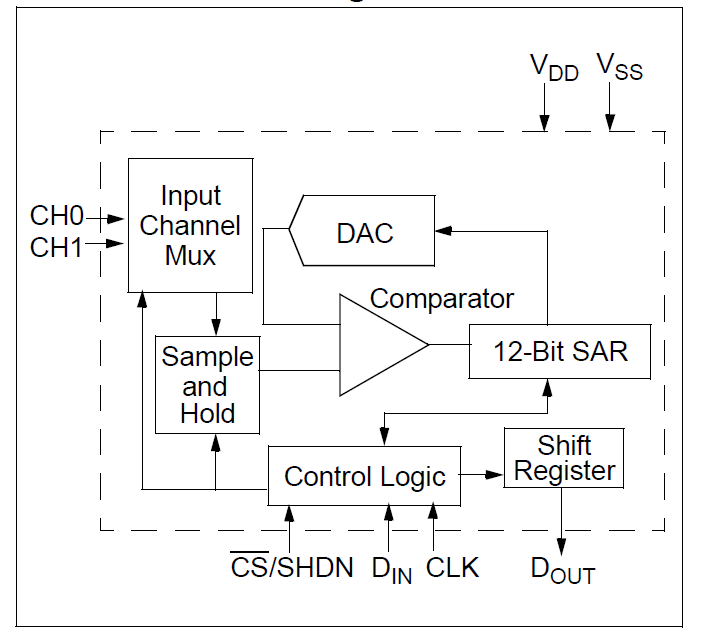
\includegraphics[width=0.5\textwidth]{adc}
\caption{Aufbau des ADC's}
\end{figure}

\
\

\subsubsection{Mikrocontroller}
Als zentrale Steuereinheit des Sensorprints haben wir einen Arduino Nano Board mit einem Atmega 328 Chip ausgewählt. Dieses Board wurde gewählt, weil in vorgängigen Projekten bereits damit gearbeitet wurde. Als Verbesserung könnte man den Atmega 328 und seine Grundbeschaltung direkt auf den Print bestücken. Somit könnte man mehr Platz sparen und den Print noch komprimierter herstellen.

Die Aufgabe des Mikrocontrollers auf dem Sensorprint beruht im allgemeinen darauf, die Verbindung zwischen dem ADC und dem Powerline Transceiver herzustellen. Die Verbindung zwischen Mikrocontroller und ADC wird mit SPI Kommunikation hergestellt. Die Verbindung zum Powerline Transceiver wird über UART Kommunikation hergestellt. Detailiertere Informationen zur Kommunikation der einzelnen Elemente untereinander sind im Abschnitt 4.1 unter Software vorhanden.


\clearpage

\subsubsection{Adressierung}
Um das Pannel identifizeren zu können, wurde Hardware basierend eine binäre Adressierung hergestellt. Diese erfolgt über einen binären 8 Bit Wert, welcher mit Dip - Switch Schaltern eingestellt werden kann. Dieser wird parallel an 8 Eingängen am Mikrocontroller eingelesen. Mit 8 Schaltern können somit 256 Pannels adressiert werden. Die Beschaltung der Schalter ist in der nachfolgenden Abbildung ersichtlich.

\begin{figure}[h]
\centering
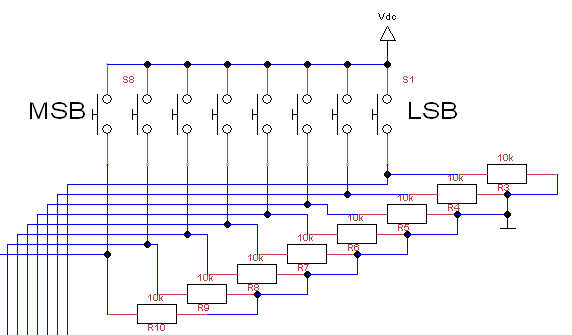
\includegraphics[width=0.7\textwidth]{adressierung}
\caption{Beschaltung der Schalter}
\end{figure}

\
\

\subsubsection{Transceiver}
Für die modelierung der Daten der Solarpannels, benutzen wir einen ST7540 Powerline Transceiver. Dieser empfängt vom Mikrocontroller über den TxD Eingang ein Signal. Dieses Signal wird intern mit frequency shift keying (FSK) modeliert. Das modelierte Signal wird an den Ausgang übertragen und mittels induktiver Einkopplung auf die Powerline eingekoppelt. Die Einkopplung erfolgt mittels einem Draht, welcher um einen Feritkern gewickelt wurde. Dieses Zusammenspiel erzeugt eine Induktion und ermöglicht somit die Einkopplung auf die Pwoerline.

\clearpage

\begin{figure}[h]
\centering
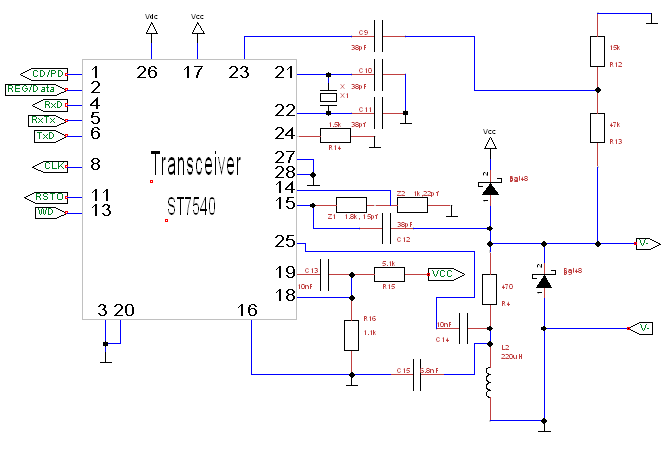
\includegraphics[width=1\textwidth]{transceiver}
\caption{Beschaltung des Transceiver}
\end{figure}


%\subsubsection{Layout}
